\svnid{$Id: bausteinsicht.tex 180 2012-05-24 15:26:04Z dgens001 $}
\chapter{Bausteinsicht}
\textit{In diesem Abschnitt soll die Struktur der Spiele-Software dargestellt werden.
Im Vordergrund stehen die Bausteine, deren Beziehungen und eine Übersicht darüber mit welchen
Klassen und Paketen die zuvor erarbeiteten Anforderungen umgesetzt werden. Die Übersicht wird
dabei schrittweise verfeinert.}



\section{Übersicht}
Das \gls{Spiel} ist grundlegend in drei Schichten eingeteilt, Darstellungs-, Logik- und 
Datenschicht. Die genauen Zusammenhänge werden im Folgenden erläutert und durch das unten stehende 
Schichten-Diagramm sowie die angehängte UML-"Tapete" verdeutlicht.


\
\\
\begin{figure}[h]
	\begin{center}
		%trim option's parameter order: left bottom right top , clip = true
		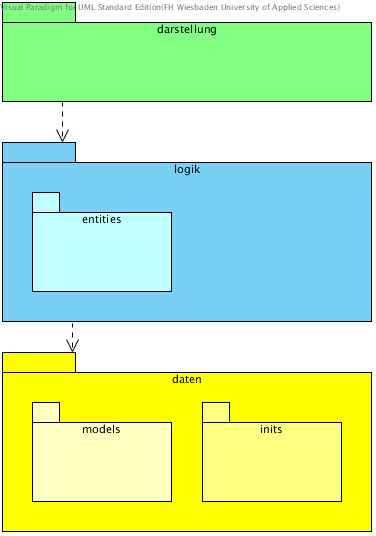
\includegraphics[height=7cm]{kapitel/bausteinsicht/schichten.png}
	\end{center}
	\caption{Architekturdiagramm}
	\label{fig:domain_uml}
\end{figure}



\section{Darstellung}
Die Darstellungsschicht beinhaltet verschiedene Klassen, die im Zusammenspiel letztlich die 
\gls{Anzeige} füllen. Die benötigte Kommunikation erfolgt dabei jeweils über 
\textit{PropertyChangeListener}, sodass Klassen der Logikschicht deren Pendants der 
Darstellungsschicht benachrichtigen können.

\
\\
\begin{figure}[h]
	\begin{center}
		%trim option's parameter order: left bottom right top , clip = true
		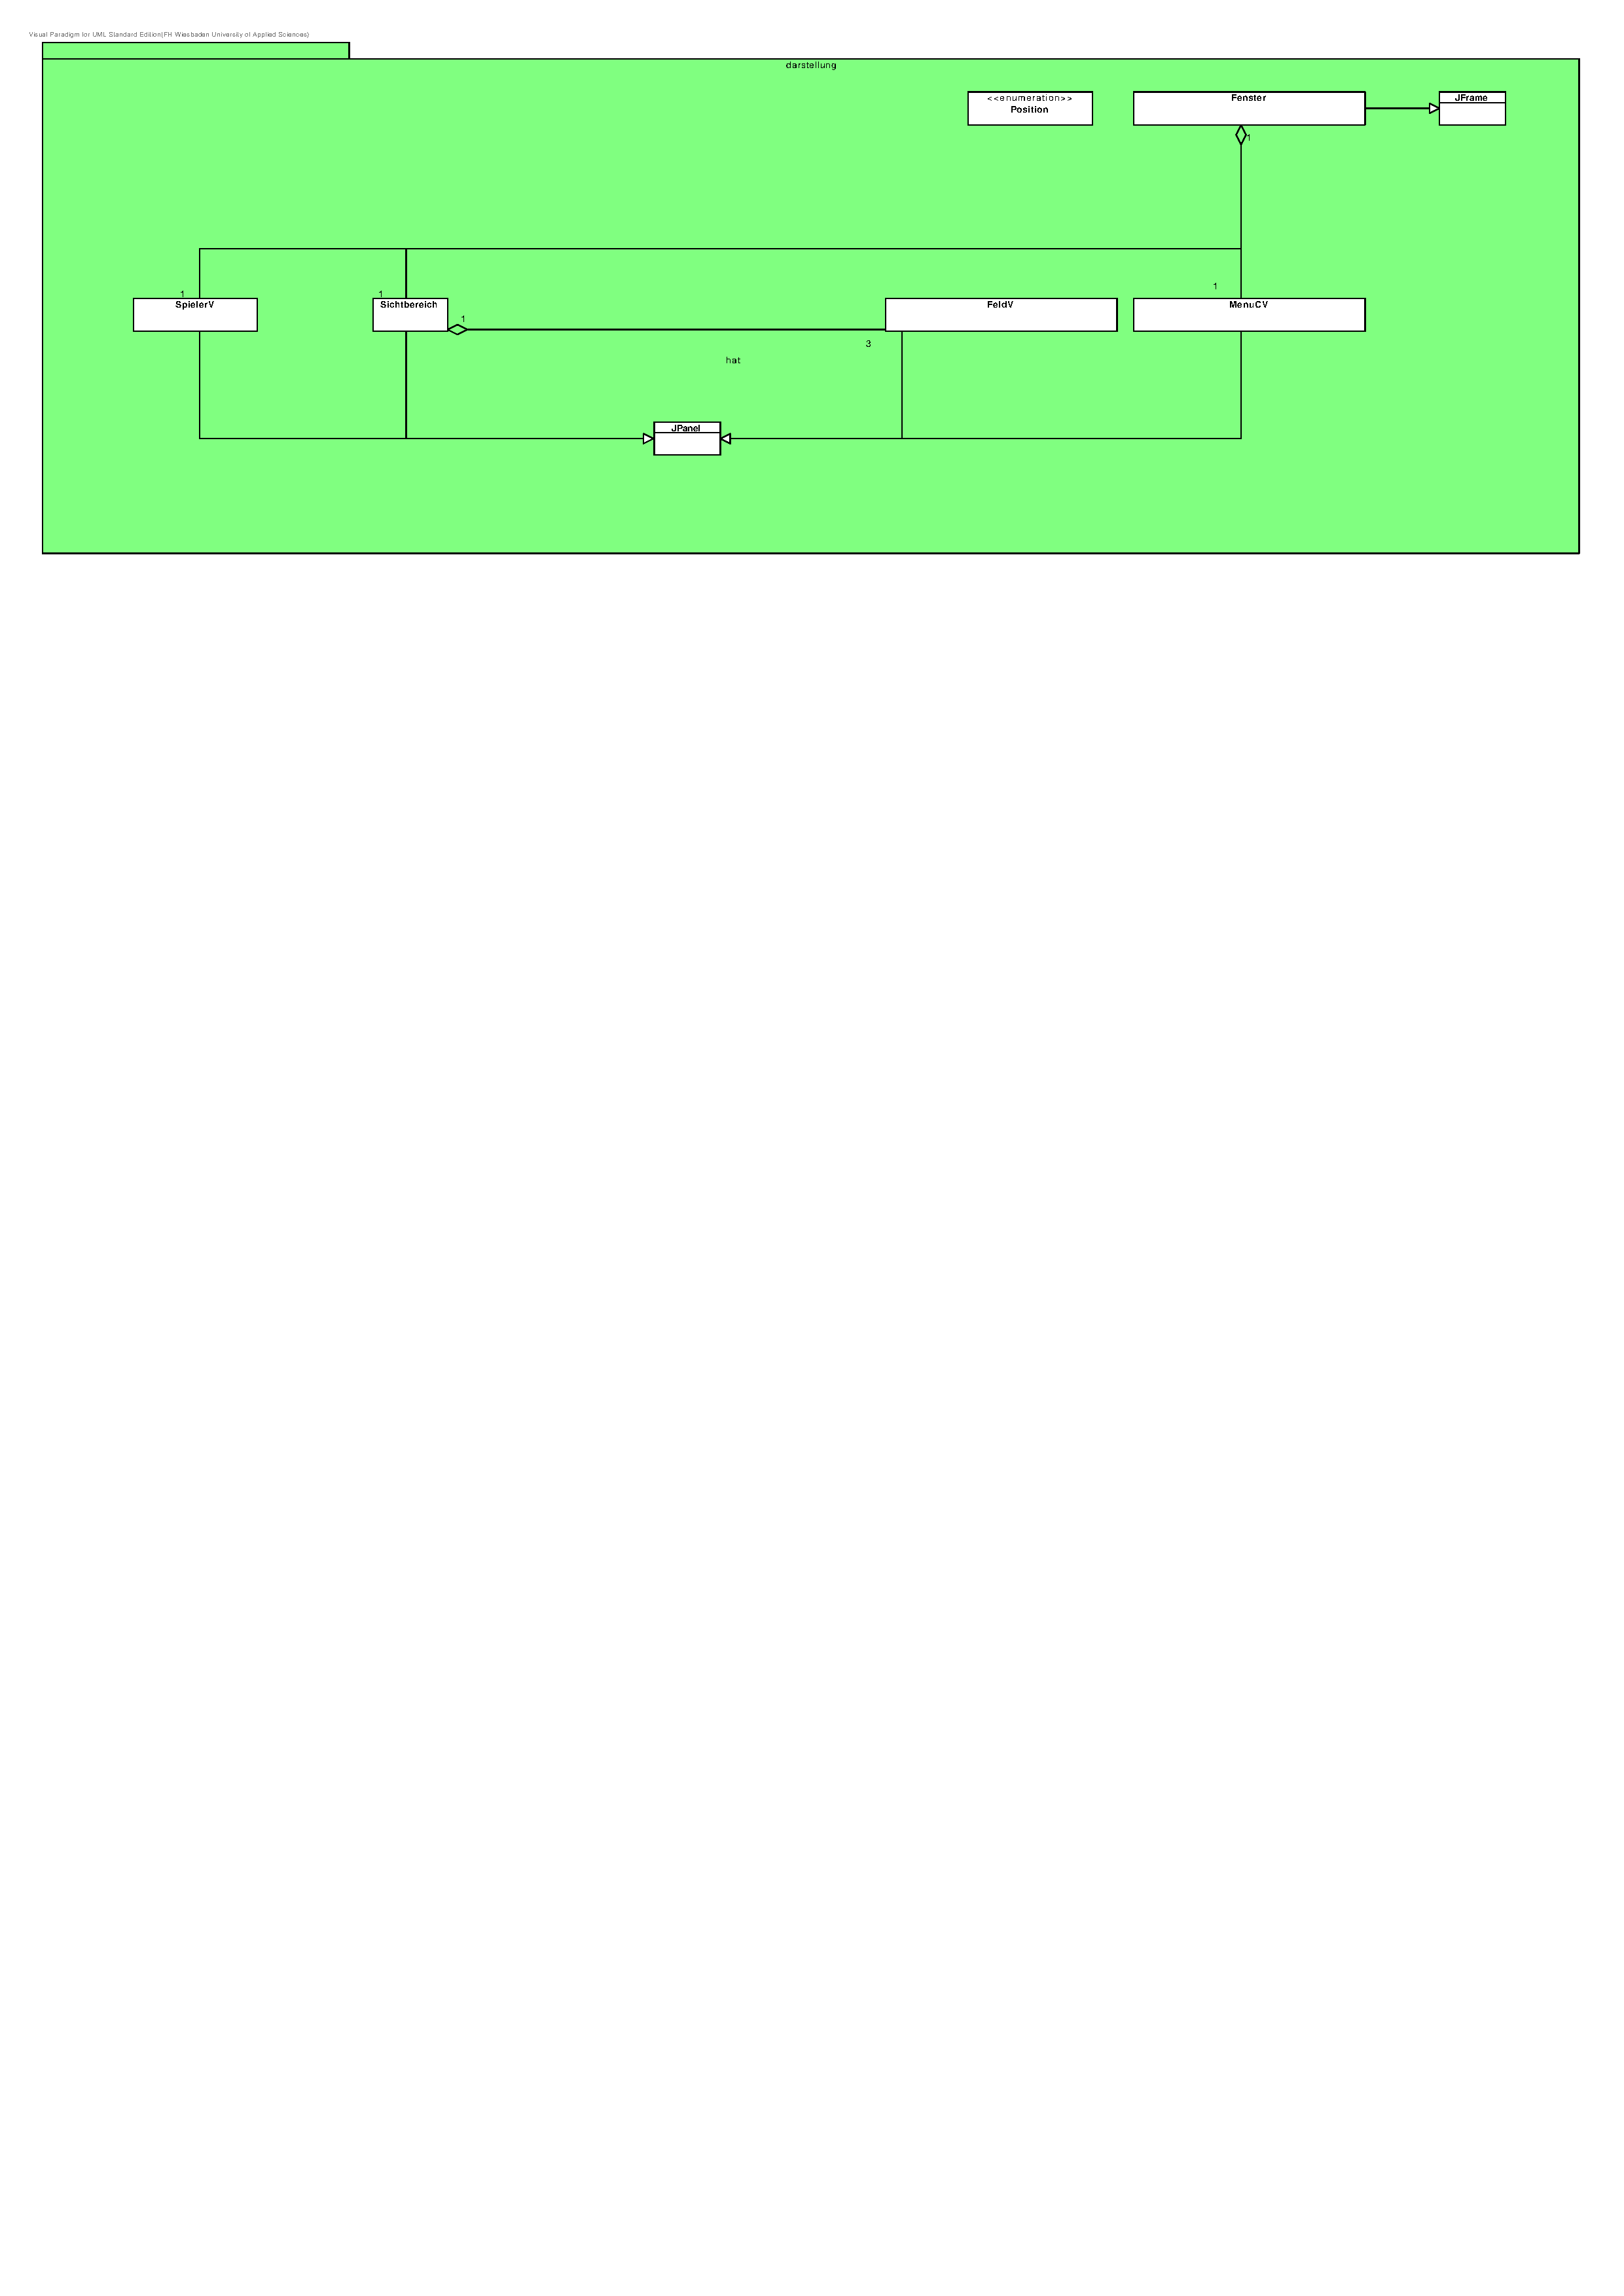
\includegraphics[trim=0cm 45cm 0cm 0cm, clip=true, width=16cm]{kapitel/bausteinsicht/darstellung.pdf}
	\end{center}
	\caption{Darstellungsschicht}
	\label{fig:darstellung_uml}
\end{figure}

\subsection{Fenster}
Das Fenster erweitert das Java \textit{JFrame} und zeigt die beiden Bereiche \gls{Statusbereich} 
(SpielerV) und \gls{Sichtbereich} (Szene) an. Falls sich der \gls{Spieler} in einem Menu befindet, 
zeigt das Fenster statt der beiden o.g. Bereiche nur das passende Menu (MenuCV) an.

\subsection{MenuCV}
Der \gls{Menuemodus} bietet dem \gls{Spieler} verschiedene Optionen an. Das Menu unterscheidet 
zudem selbst, welches Untermenu gezeigt wird. Dazu stehen z.B. die Funktionen \textit{drawPause()} 
oder \textit{drawSave()} bereit.

\subsection{Sichtbereich}
Der \gls{Sichtbereich} zeigt die \gls{Welt} in einer Pseudo-3D-Perspektive an. Es werden dabei immer 
die nächsten drei \glspl{Feld} in \gls{Blickrichtung} des \gls{Spieler}s mit ihren \glspl{GameObject} 
dargestellt. Die anderen Felder eines Raumes werden ohne evtl. \glspl{GameObject} gezeigt.

Die Darstellung der Felder mit \glspl{GameObject} erfolgt über drei \textit{FeldV}, welche die drei 
vorderen \glspl{Feld} in \gls{Blickrichtung} des \gls{Spieler}s darstellen. Diese werden von 
\textit{Sichtbereich} mit dem darzustellenden Feld und der benötigten Position des \gls{Feld}es 
(vorne, mitte, hinten).

Alle anderen \textit{JPanels} des \gls{Sichtbereich}s werden je nach Position des \gls{Spieler}s und 
dessen \gls{Blickrichtung} mit verschiedenen Texturen versehen, sodass ein räumlicher Eindruck entsteht.

\subsection{FeldV}
Die eigentliche Darstellung von \glspl{GameObject} auf den drei vorderen \glspl{Feld} wird von 
\textit{FeldV} übernommen, welches ein Raster anzeigt.

Dieses Raster zeigt die einzelnen \gls{Item}-, \gls{npc}- und \gls{Eingang}sanordnungen des 
\gls{Feld}es. Dazu wird die \textit{getObjects}-Methode der \gls{Feld}-Klasse vom View aufgerufen. 
Rückgabe ist hierbei eine Liste von \glspl{GameObject}, von welchen mit \textit{getImg()} deren 
Bild und evtl. Name angezeigt werden kann.

\subsection{SpielerV}
Der \textit{SpielerV} zeigt die Statusleiste an. Diese wird je nach Bedarf mit den passenden Inhalten 
gefüllt. Es wird z.B. das \gls{Inventar} und der Avatar des \gls{Spieler}s gezeigt. Tritt der 
\gls{Spieler} in Interaktion mit einem \gls{GameObject}, wird auch dazu der passende View gewählt. 
Die Auswahl erfolgt mit Hilfe der Funktionen \textit{drawInventar()}, \textit{drawInteraktion()}, 
\textit{drawHand()} und \textit{drawAvatar()}. Was zu tun ist, wird von \textit{Spieler} durch ein 
\textit{PropertyChangeEvent} angestoßen.

\paragraph{Infobereich}
Im \gls{Infobereich} werden je nach Situation das \gls{Inventar} des \gls{Spieler}s mit dessen Slots 
und den darin befindlichen \glspl{Gegenstand}n gezeigt oder textuelle Information bei Interaktionen 
dargestellt.

\paragraph{Handbereich}
Wählt der \gls{Spieler} die Interaktion mit einem \gls{Gegenstand} wird im \gls{Handbereich} das 
Bild des jeweiligen \gls{Item}s angezeigt. Im Normalfall wird eine leere Hand gezeigt.

\paragraph{Statusbereich}
Im \gls{Statusbereich} kann der \gls{Spieler} verschiedene Informationen zu sich selbst oder einem 
\gls{npc} erhalten. Meist wird ein Portät des jeweiligen Charakters dargestellt.

\subsubsection{Interaktion}
Die Methode \textit{drawInteraktion()} unterscheidet zudem den Typ des gewählten \gls{GameObject}s 
und füllt \gls{Infobereich}, \gls{Statusbereich} und \gls{Handbereich} mit den nötigen Inhalten. 

\paragraph{Interaktion mit Gegenständen}
% interaktion mit objekt
Bei der Interaktion mit einem \gls{Gegenstand} wird dessen Beschreibung und die möglichen 
Interaktionen, die der \gls{Spieler} damit tätigen kann, angezeigt. Er kann diese beispielsweise 
in sein \gls{Inventar} aufnehmen. Nimmt der \gls{Spieler} einen \gls{Gegenstand} auf, wird er zuerst 
in der Hand "zwischengespeichert". Das Bild des \gls{Gegenstand}s wird daher im \gls{Handbereich} 
angezeigt.

\paragraph{Interaktion mit NPCs}
Spricht der \gls{Spieler} hingegen einen \gls{npc} an, werden im \gls{Statusbereich} dessen Bild und 
Name gezeigt. Anhand des \textit{\gls{Dialog}Model}, stellt \textit{SpielerV} den \gls{Dialog} mit 
Text, Antworten und evtl. einem \gls{Item} dar, welches der \gls{Spieler} durch den letzten 
\gls{Dialog} erhalten hat.

\subsubsection{Inventar}
Der \gls{Spieler} besitzt ein \gls{Inventar} mit 10 Slots und eine \textit{Hand}. Diese kann 
lediglich einen einzigen \gls{Gegenstand} aufnehmen und dient als "Zwischenspeicher" bei einer 
Interaktion. Dargestellt werden \gls{Inventar} und Hand jeweils von \textit{drawInventar()} und 
\textit{drawHand()} der Klasse \textit{SpielerV}. Über den \glspl{Gegenstand}n im \gls{Inventar} 
werden Nummern angezeigt, die auf den passenden Index verweisen. Drückt der \gls{Spieler} eine 
dieser Nummern, wird der \gls{Gegenstand} aus dem \gls{Inventar} in die Hand genommen und beide 
Bereiche neu gezeichnet.
\newpage


\section{Logik}
In der Logik-Schicht befinden sich das Paket \textit{entities} und die Controller \textit{TastaturC} 
und \textit{GameC}.

Die hierin befindlichen Klassen sind jeweils möglichst autark - jegliche Funktionen, Interaktionen 
oder mögliches Zusammenspiel zwischen den Klassen/Objekten geschieht ohne Zutun einer dritten 
Instanz.

Ein Beispiel: Möchte der \gls{Spieler} einen \gls{Gegenstand} aufnehmen, wird die gesamte Logik vom 
\gls{Spieler} selbst übernommen - es gibt keine extra Klasse, die sich um den Ablauf kümmert. Zur 
Kommunikation zwischen den Klassen wird das Interface \textit{interagiere} verwendet.

\begin{figure}[h]
	\begin{center}
		%trim option's parameter order: left bottom right top , clip = true
		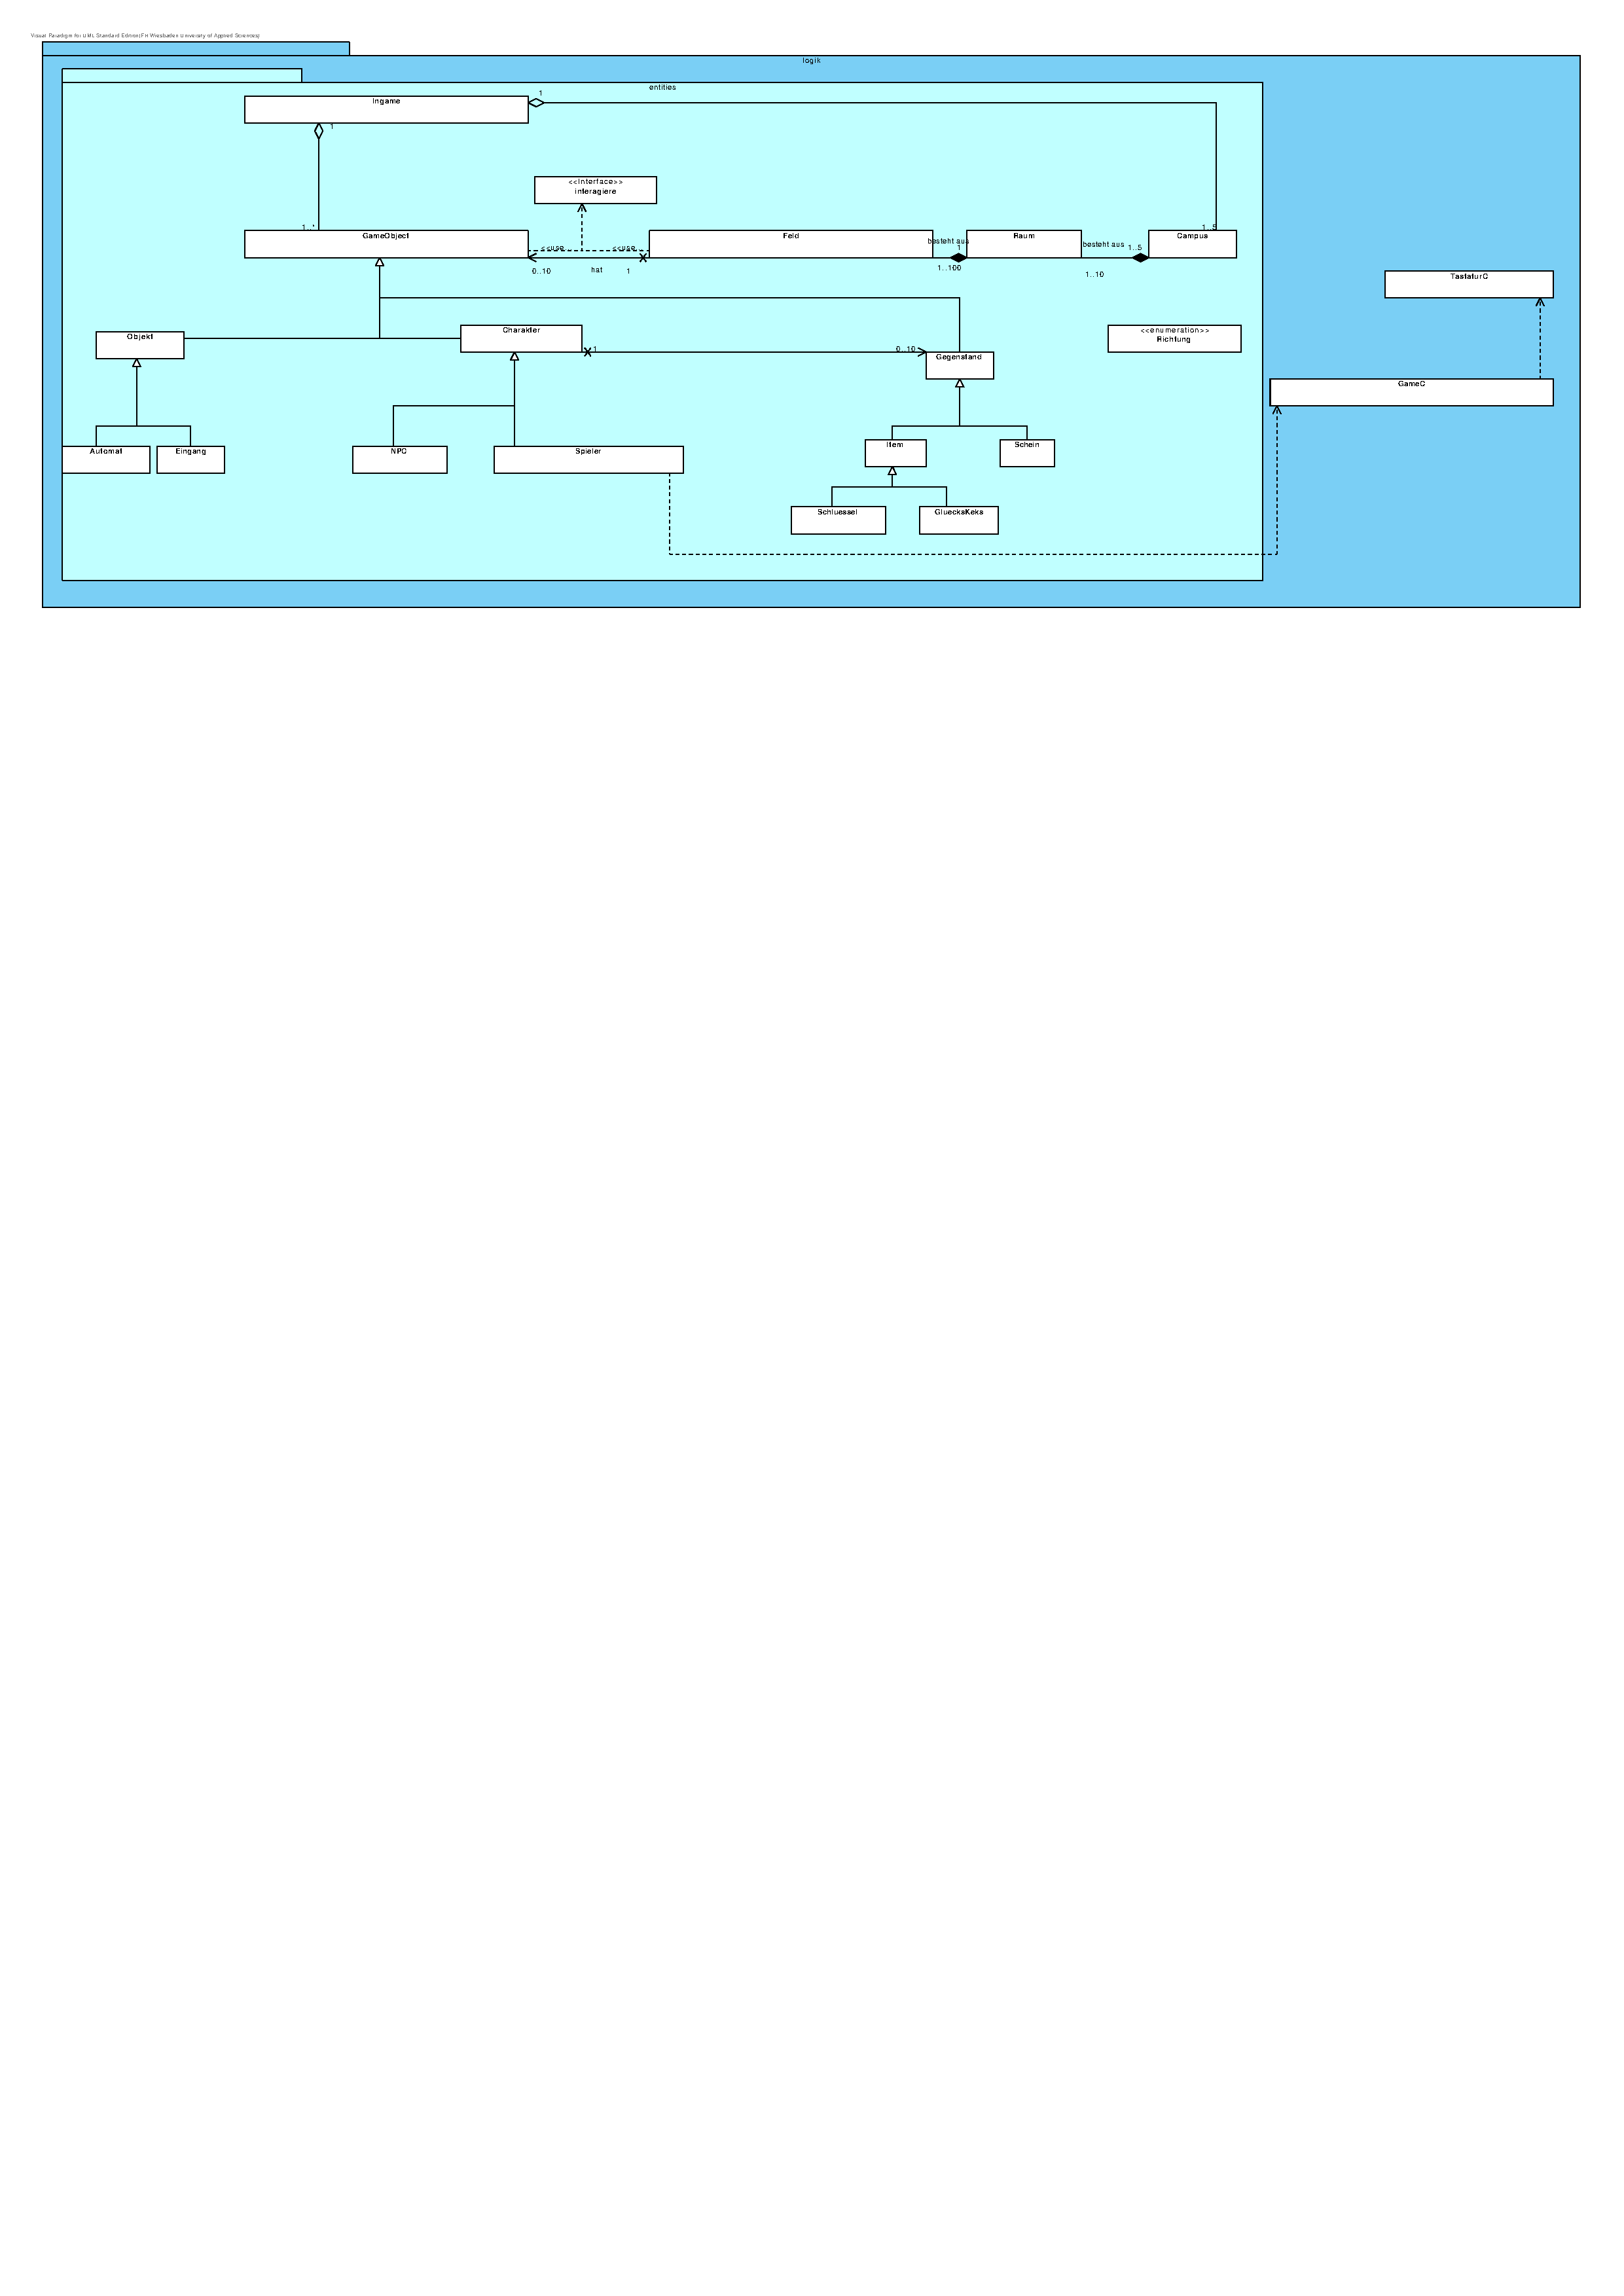
\includegraphics[trim=0cm 43cm 0cm 0cm, clip=true, width=16cm]{kapitel/bausteinsicht/logik.pdf}
	\end{center}
	\caption{Logikschicht}
	\label{fig:logik_uml}
\end{figure}

\subsection{Entities}
Das Paket \textit{entities} umfasst alle Klassen, die autark Funktionen erfüllen. Die evtl. 
benötigten Models sind im Paket \textit{models} der Datenschicht ausgelagert. Es wird hierbei das 
MVC-Pattern verwendet, um eine saubere Trennung zu gewährleisten.

\paragraph{Ingame}
Das \textit{Ingame}-Objekt beinhaltet Referenzen zu allen anderen Objekten des \textit{entities} 
Pakets. Das hat den Vorteil, dass beim Speichern nur dieses Objekt serialisiert werden muss und alle 
anderen Objekte automatisch mit gespeichert werden.

\paragraph{Feld}
Das \textit{Feld} bildet die zentrale Anlaufstelle für \textit{Spieler} und \textit{FeldV}, sodass 
es möglich ist, \glspl{Gegenstand} aufzunehmen, abzulegen und anzuzeigen. Die Kommunikation läuft 
über das Interface \textit{interagiere}.

\paragraph{Raum}
Der \gls{Raum} grenzt eine Menge von \glspl{Feld}n ein und macht sie zugänglich oder nicht. Hierdurch 
ist es beispielsweise möglich, dass der \gls{Spieler} nur \glspl{Raum} betritt, für die er einen 
Schlüssel bei sich trägt.

\paragraph{Campus}
Der \gls{Campus} umfasst alle \glspl{Raum} und grenzt die \gls{Welt} ein. Der \gls{Spieler} kann sich 
nur innerhalb eines \gls{Campus} bewegen.

\paragraph{GameObject}
Die Klasse \gls{GameObject} stellt die grundlegende Klasse für alle in der \gls{Welt} lebenden \glspl{Objekt}
dar. \glspl{GameObject} haben einen Namen und eine textuelle Beschreibung sowie ein Bild (an Stelle eines
eigenen Views).

\paragraph{Charakter}
\gls{Charakter} sind menschliche Spielfiguren, die ein eigenes \gls{Inventar} haben (also \glspl{Gegenstand}
aufnehmen können) und mit mit anderen \glspl{Charakter}n in \gls{Dialog} treten können.

\paragraph{NPC}
\gls{npcs} sind vom Computer gesteuerte \glspl{Charakter}, die zusätzlich einen \textit{Dialog} haben.
	
\paragraph{Spieler}
Die \textit{Spieler}-Klasse ist zentrales Objekt im \gls{Spiel}, denn sie stellt die virtuelle Repräsentation
des menschlichen \gls{Spieler}s dar. Jegliche Art von Interaktion wird von \gls{Spieler} (über das
\textit{interagiere}-Interface) angestoßen. Zusätzlich kann der \gls{Spieler} sich bewegen.

\paragraph{Gegenstand}
\glspl{Gegenstand} sind \glspl{Objekt} die der \gls{Spieler} aufnehmen kann. \glspl{Gegenstand} liegen z.B. auf
\glspl{Feld}n. Aber auch \glspl{Charakter} können dem \gls{Spieler} \glspl{Gegenstand} im Verlauf eines 
\gls{Dialog} überreichen. \glspl{Gegenstand} können beliebig spezialisiert sein und so zum Spielinhalt
beitragen.

\paragraph{Objekt}
Objekte sind im Gegensatz zu Gegenständen nicht aufnehmbar. Sie belegen aber einen Slot auf dem jeweiligen
Feld. Ein Beispiel für ein spezialisiertes Objekt ist der Automat, welcher bei Interaktion Gegenstand liefert.

\paragraph{Eingang}
\textit{Eingang} ist ein \textit{Objekt} und kann offen oder verschlossen sein und ist mit einem passenden
\textit{Schlüssel} aufschließbar.

\paragraph{Richtung}
Ein Enum um die \gls{Blickrichtung} des \gls{Spieler}s zu definieren. Wird z.B. von Klassen der
Darstellungsschicht verwendet, um die korrekten \glspl{Feld} im \gls{Sichtbereich} des \gls{Spieler}s
zu finden.

\subsection{Controller}
Die Controller liegen in der Logikschicht, verwenden aber kein eigenes Package. Sie kümmern sich um 
den Wechsel der Ansichten (Menu, Ingame) und um Tastatureingaben des \gls{Spieler}s.

\paragraph{TastaturC und GameC}
Zur Eingabe über die Tastatur hört \textit{TastaturC} und leitet die Eingaben an \textit{GameC} 
weiter. \textit{GameC} benachrichtigt dann, abhängig davon ob gerade ein Menu angezeigt wird oder 
nicht, die passende Klasse (\textit{Spieler} oder \textit{MenuCV}) via \textit{PropertyChangeEvent}.

\newpage

\section{Daten}
Die Datenschicht beinhaltet die Pakete \textit{models} und \textit{init}.
Hier befinden sich alle Klassen, die selbst keine direkten Spiel-Funktionen anbieten. Meist werden 
die Models durch entsprechende Factories aus Konfigurationsdateien erstellt und stehen dann Klassen 
aus der Logikschicht zur Verfügung.

\begin{figure}[h]
	\begin{center}
		%trim option's parameter order: left bottom right top , clip = true
		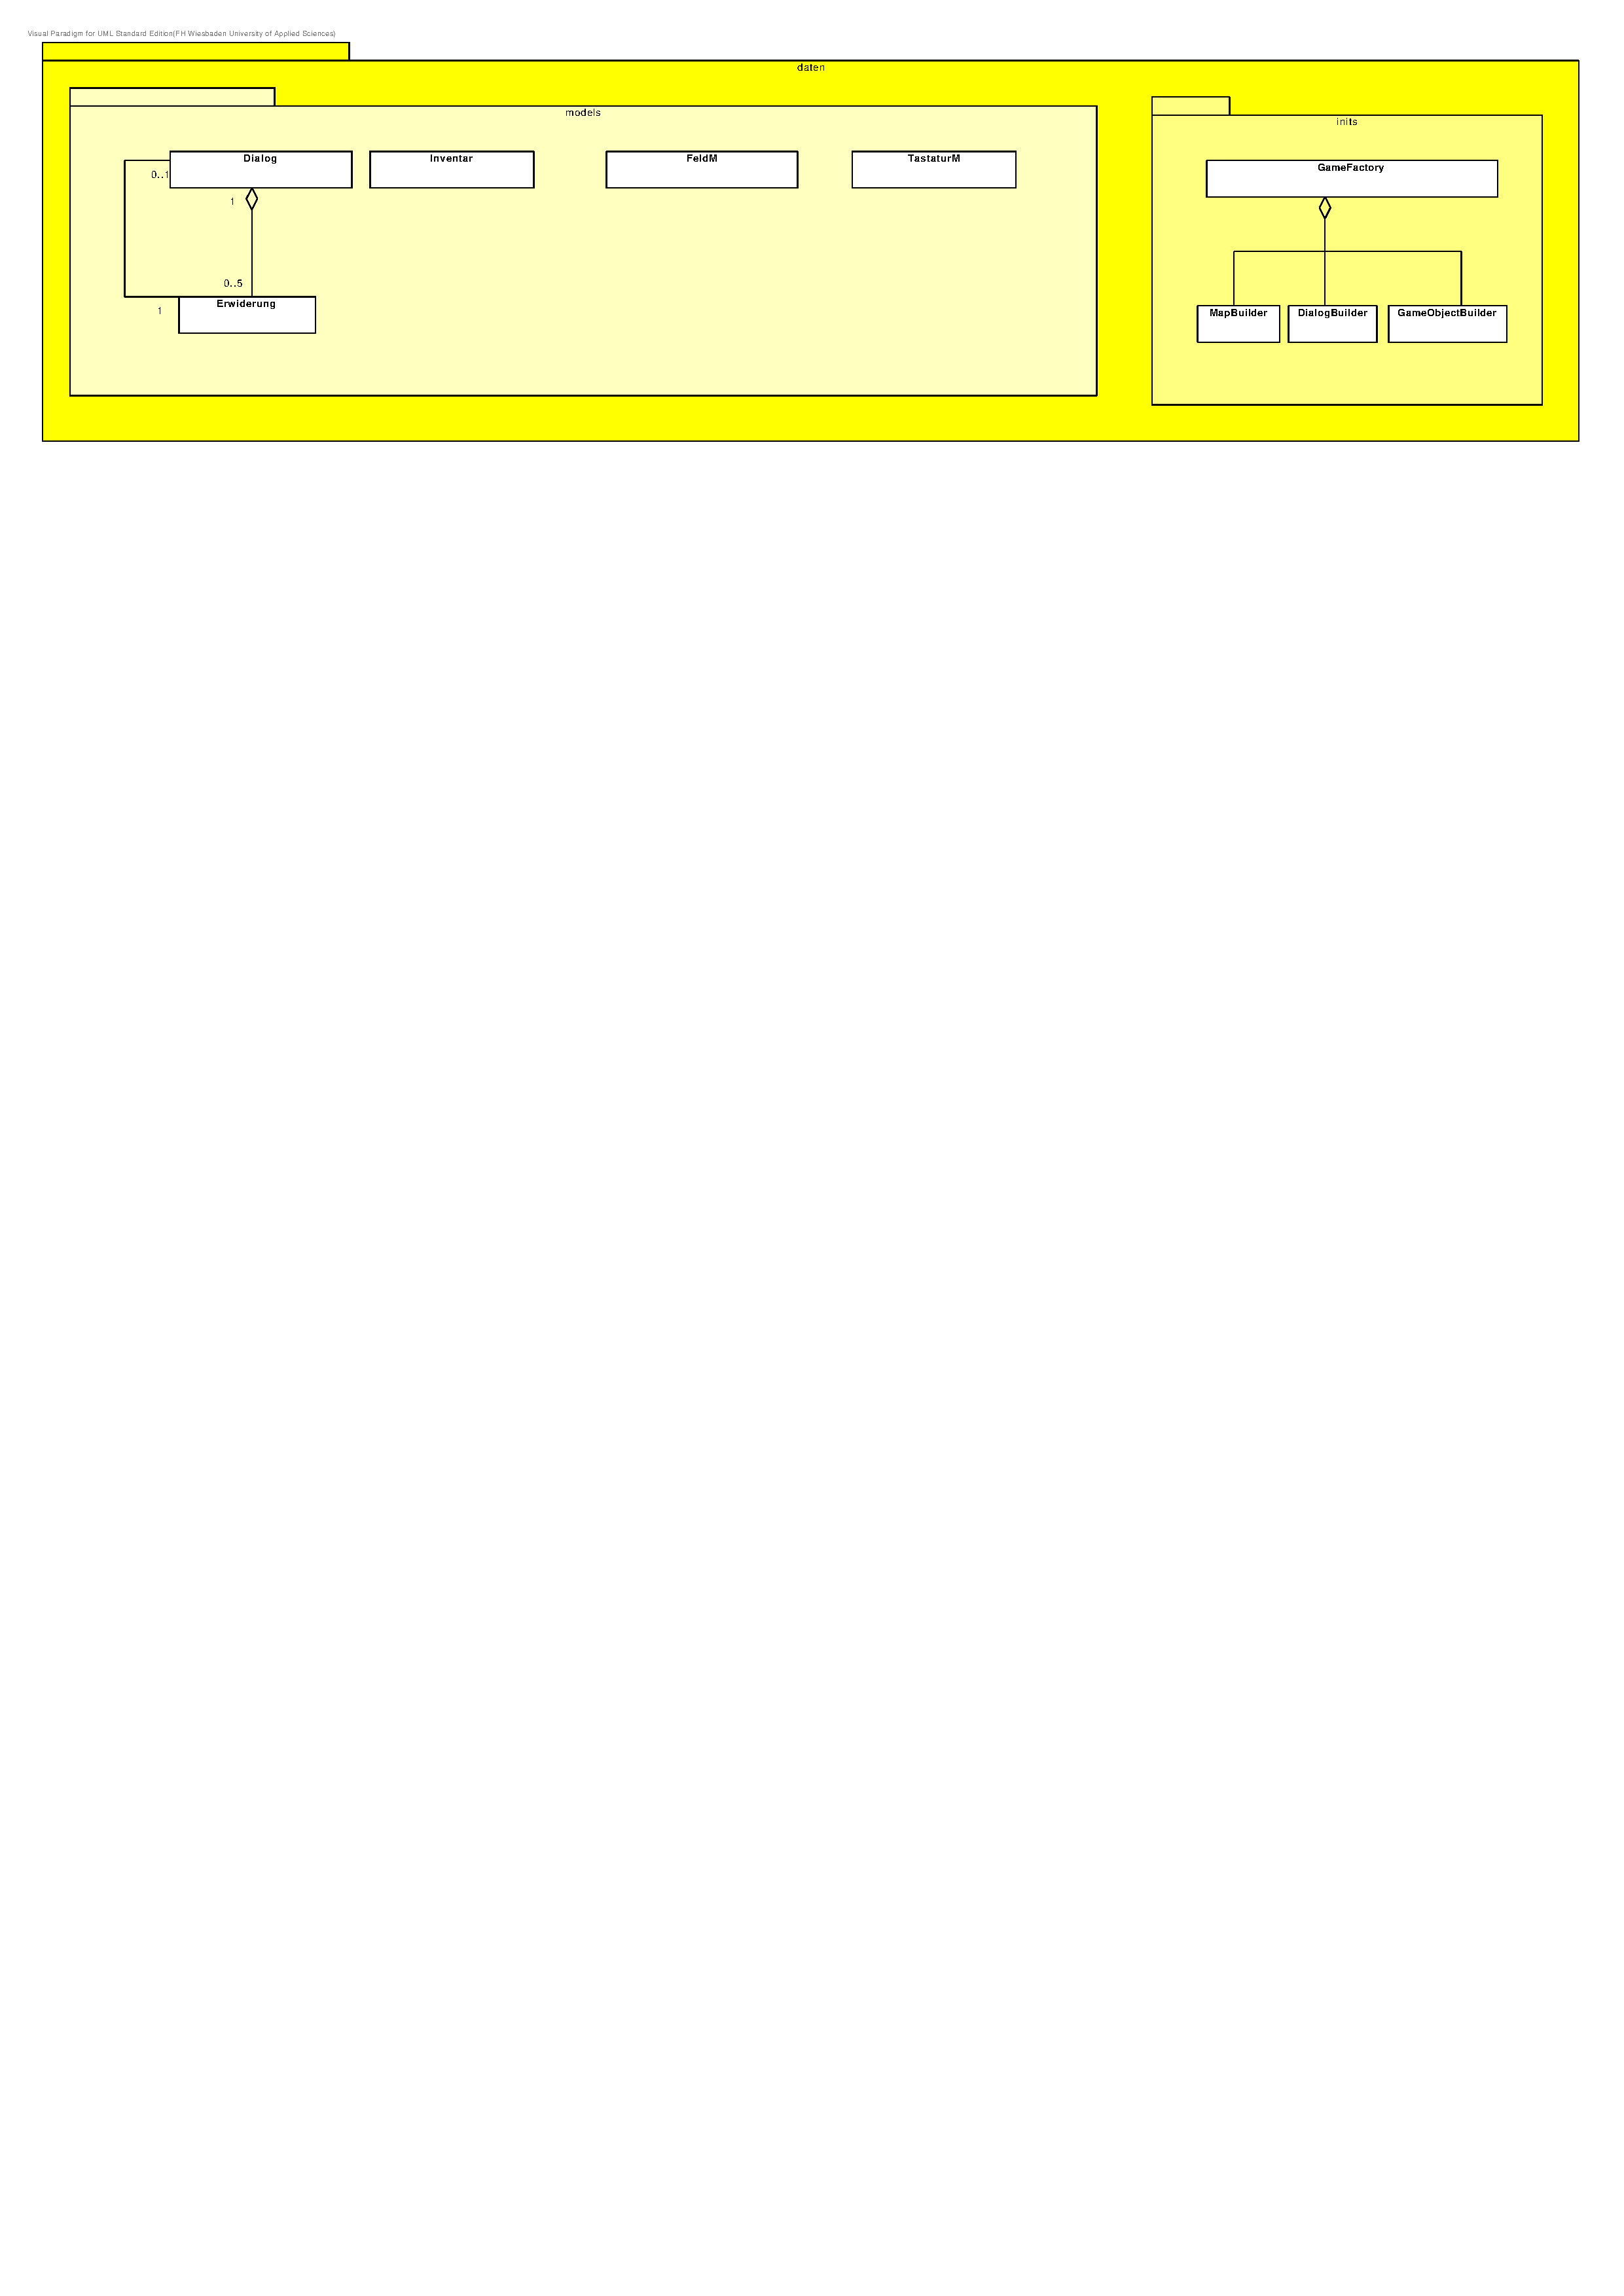
\includegraphics[trim=0cm 45cm 0cm 0cm, clip=true, width=16cm]{kapitel/bausteinsicht/daten.pdf}
	\end{center}
	\caption{Datenschicht}
	\label{fig:daten_uml}
\end{figure}

\paragraph{Dialog und Erwiderung}
Die Dialoge bilden das Rückgrat der Interaktion mit \gls{npcs}. Der Gesprächsablauf wird dabei
allerdings von Klassen in der Logikschicht übernommen. Dialoge beinhalten daher nur Referenzen zu
Erwiderungen und evtl. Geschenken, die der \gls{Spieler} erhält. Stößt der \gls{Spieler} auf einen 
\gls{Dialog}, werden ihm mögliche Erwiderungen angeboten, die er 
wählen kann. Jede Erwiderung leitet dabei auf einen neuen \gls{Dialog} oder auf das Ende der 
Unterhaltung.

\paragraph{Inventar}
Das \textit{Inventar} bietet nur rudimentäre Funktionen zum Füllen und Entnehmen von 
\glspl{Gegenstand} und wird einem \gls{Charakter} als Model mitgegeben.

\paragraph{FeldModel}
Jedes \gls{Feld} aus der Logikschicht erhält ein \textit{FeldM}, welches alle nötigen Daten aufnimmt 
und rudimentäre Funktionen (z.B. ob das \gls{Feld} begehbar ist) anbietet. Möchte der \gls{Spieler} 
einen \gls{Gegenstand} aufnehmen oder ablegen, werden diese ähnlich zu einem \gls{Inventar} im 
\textit{FeldModel} verwaltet.

\paragraph{Factories und Builder}
Die Klassen im Paket \textit{init} sind hauptsächlich Factories, die die benötigten Models aus 
Konfigurationsdateien erstellen und die passenden Models bereitstellen.
